% ESP32-C61 two-bank SRAM handoff, based on direct_iq_test/doc/two_bank_iq_sram.md.
% Banks are reserved with SOC_RESERVE_MEMORY_REGION; ownership is switched only
% after the dump write pointer leaves a bank. This is not the C5/S3 snapshot path
% or the separate PSRAM stream-frame queue in main/ringbuffer.c.
% Build: pdflatex iq-ring-buffer.tex; pdf2svg iq-ring-buffer.pdf iq-ring-buffer.svg
\documentclass[border=5pt]{standalone}
\usepackage{helvet}
\renewcommand{\familydefault}{\sfdefault}
\usepackage{tikz}
\usetikzlibrary{arrows.meta,calc,positioning}
\definecolor{accent}{HTML}{37C964}
\definecolor{surface}{HTML}{293135}
\definecolor{foreground}{HTML}{DEE2E6}
\definecolor{muted}{HTML}{ADB5BD}
\definecolor{outline}{HTML}{66757D}
\begin{document}
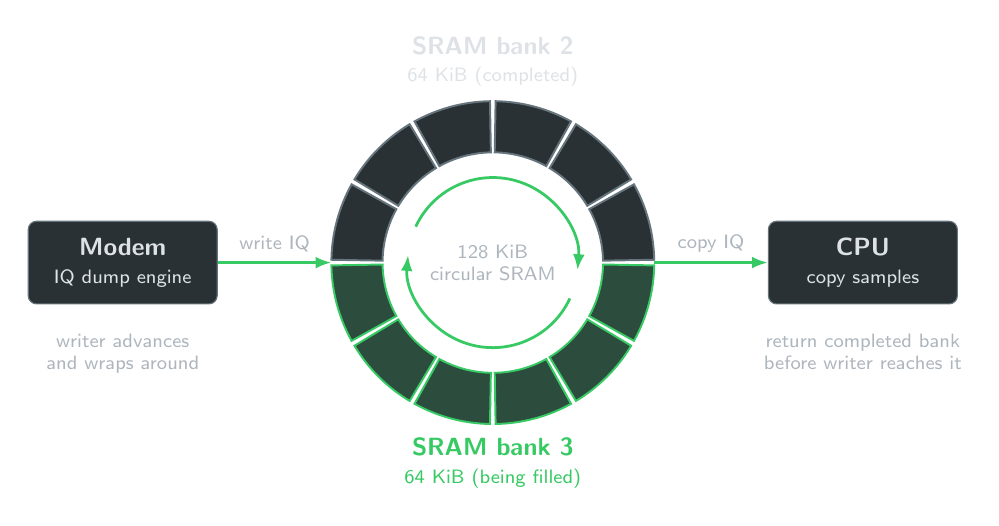
\begin{tikzpicture}[
  font=\sffamily\small, text=foreground,
  block/.style={draw=outline, fill=surface, rounded corners=3pt,
    minimum width=3.5cm, minimum height=1.05cm, align=center},
  flow/.style={-{Latex[length=2mm]}, line width=1pt, accent},
  cycleflow/.style={-{Latex[length=1.8mm]}, line width=.8pt, muted, rounded corners=6pt},
  label/.style={font=\scriptsize, text=muted, align=center}
]

  % Twelve visual sectors suggest successive sample locations, not extra banks.
  % The upper and lower semicircles are the two physical 64 KiB SRAM banks.
  \foreach \a in {0,30,...,150} {
    \path[draw=outline, fill=surface, line width=.7pt]
      (\a+1:2.05) arc[start angle=\a+1,end angle=\a+29,radius=2.05]
      -- (\a+29:1.4) arc[start angle=\a+29,end angle=\a+1,radius=1.4] -- cycle;
  }
  \foreach \a in {180,210,...,330} {
    \path[draw=accent, fill=accent!18!surface, line width=.7pt]
      (\a+1:2.05) arc[start angle=\a+1,end angle=\a+29,radius=2.05]
      -- (\a+29:1.4) arc[start angle=\a+29,end angle=\a+1,radius=1.4] -- cycle;
  }
  \node[align=center] at (0,2.55)
    {\textbf{SRAM bank 2}\\[-1pt]{\scriptsize 64 KiB (completed)}};
  \node[align=center, text=accent] at (0,-2.55)
    {\textbf{SRAM bank 3}\\[-1pt]{\scriptsize 64 KiB (being filled)}};

  \draw[flow] (155:1.08) arc[start angle=155,end angle=-5,radius=1.08];
  \draw[flow] (-25:1.08) arc[start angle=-25,end angle=-185,radius=1.08];
  \node[label] at (0,0) {128 KiB\\circular SRAM};

  \node[block, minimum width=2.4cm] (modem) at (-4.7,0)
    {\textbf{Modem}\\[-1pt]{\scriptsize IQ dump engine}};
  \node[block, minimum width=2.4cm] (cpu) at (4.7,0)
    {\textbf{CPU}\\[-1pt]{\scriptsize copy samples}};
  \draw[flow] (modem.east) -- node[label, above]{write IQ} (180:2.05);
  \draw[flow] (0:2.05) -- node[label, above]{copy IQ} (cpu.west);
  \node[label, below=.25cm of modem] {writer advances\\and wraps around};
  \node[label, below=.25cm of cpu] {return completed bank\\before writer reaches it};
\end{tikzpicture}
\end{document}
